% Data science talk by Roy Keyes and Steve Koch
% Sept. 2013

%\documentclass[11pt,hyperref={pdfpagelabels=false},xcolor=table]{beamer}
\documentclass[11pt,xcolor=table]{beamer}
\usepackage[table]{xcolor}
\usepackage{graphicx}
%\usepackage{epsfig,amsmath,amssymb,bm,epsf,graphicx,latexsym,amsfonts}



%%%%%%%%%%%%%%%%%%%%%%%%%%%%%%%%%%%%%%%%%%%%%%%%%%%%%%%%%%%%%%%%%%%%%%%%%
% Caption command for unobtrusive copyright attribution.
\newbox\mytempbox
\newdimen\mytempdimen

\newcommand\includegraphicscopyright[3][]{%
  \leavevmode\vbox{\vskip3pt\raggedright\setbox\mytempbox=\hbox{\includegraphics[#1]{#2}}%
    \mytempdimen=\wd\mytempbox\box\mytempbox\par\vskip1pt%
    \fontsize{3}{3.5}\selectfont{\color{black!25}{\vbox{\hsize=\mytempdimen#3}}}\vskip3pt%
}}

%%%%%%%%%%%%%%%%%%%%%%%%%%%%%%%%%%%%%%%%%%%%%%%%%%%%%%%%%%%%%%%%%%%%%%%%%

\title[Data Science]{\large \textbf{Data Science, Big Data, and other buzz words}}
\titlegraphic{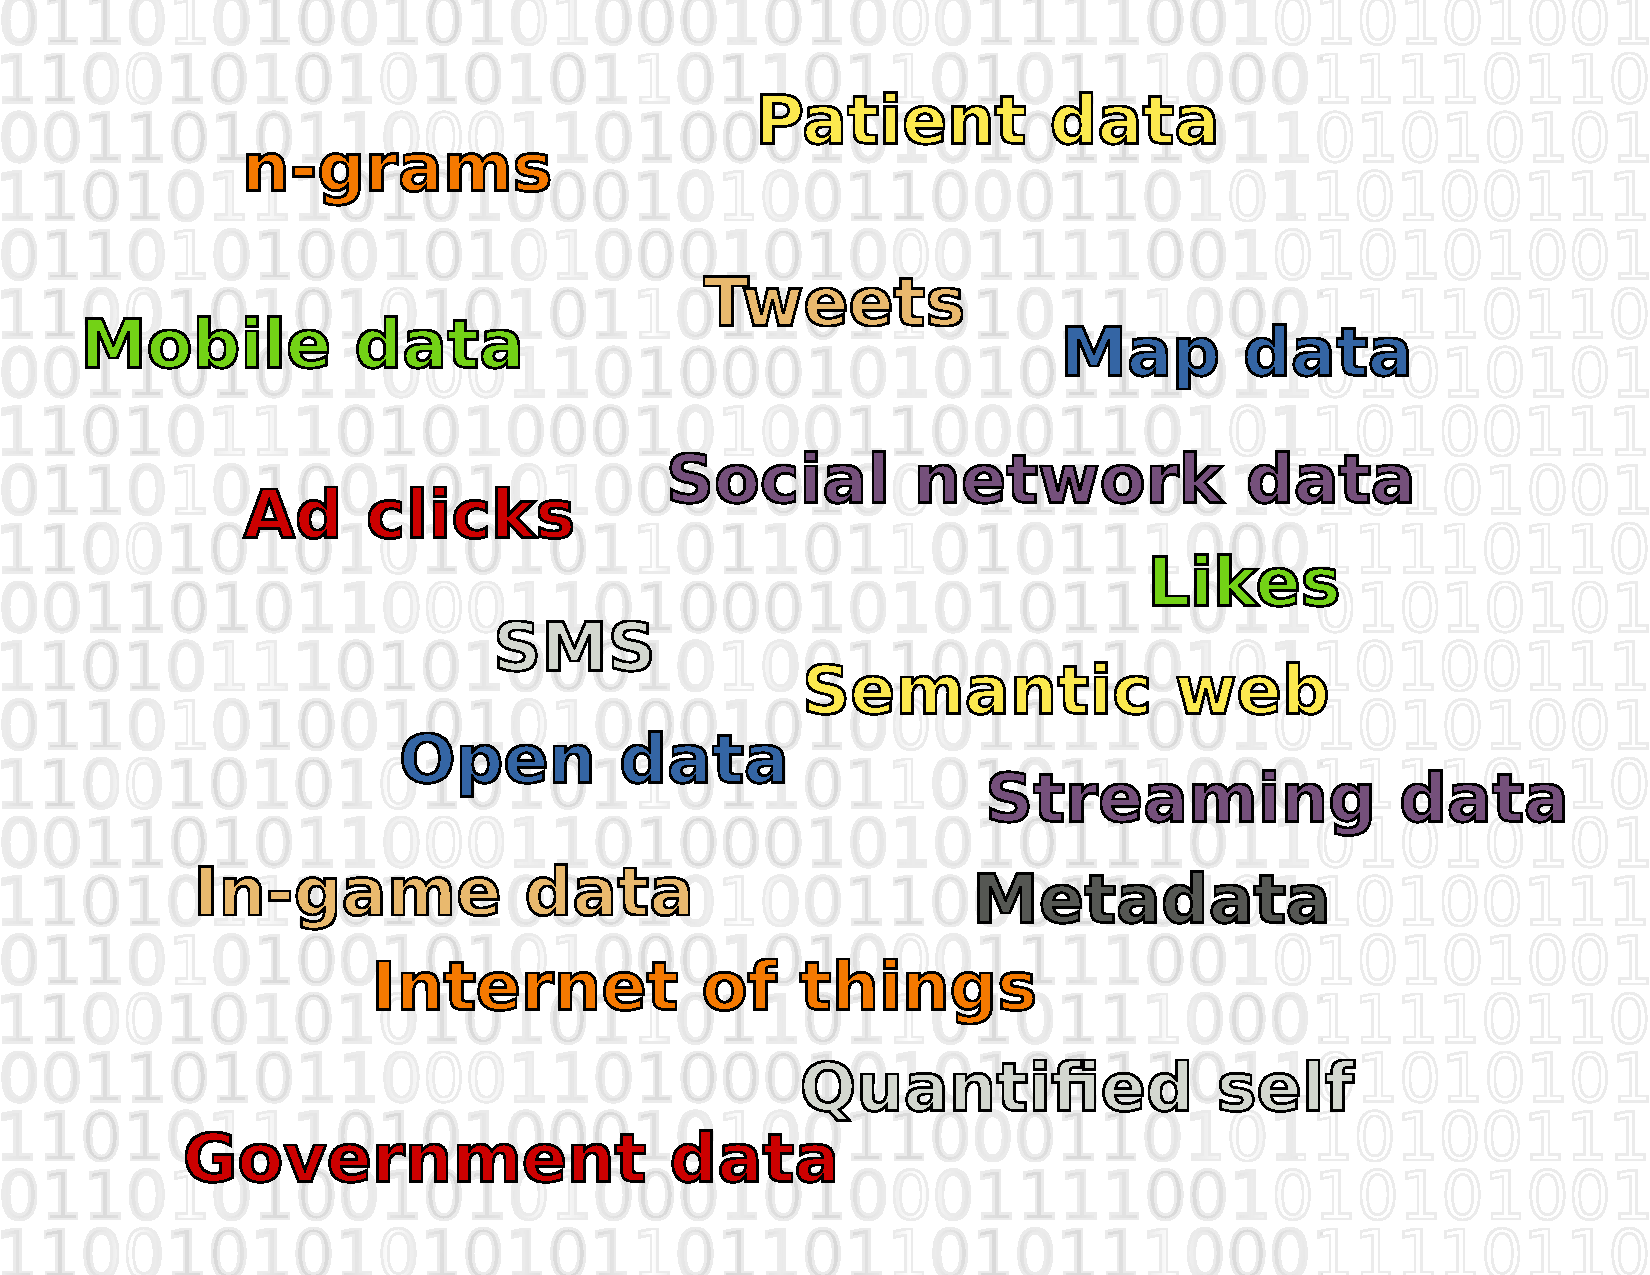
\includegraphics[width=0.6\textwidth]{graphics/data_cloud2.pdf}}
\author[Keyes and Koch]{Roy Keyes$^1$ and Steve Koch$^2$}
\institute[ZDS, UNML]{\begin{small}1. Zefs Data Science\\ 2. University of New Mexico Libraries\end{small}}
\date[13 Sept 2013]{\begin{tiny}13 Sept 2013\end{tiny}}

\mode<presentation> {
	\usetheme{Boadilla}
	\setbeamercovered{transparent}
	\useinnertheme{rectangles}
	\setbeamertemplate{blocks}[rounded][shadow=false]
	\setbeamercolor*{palette sidebar secondary}{use=structure,fg=white,bg=structure.fg!60!white}
}
\setbeamertemplate{navigation symbols}{}
\setbeamertemplate{caption}[numbered]
%\setbeamertemplate{footline}[default]
%\providecolors

%%%%%%%%%%%%%%%%%%%%%%%%%%%%%%%%%%%%%%%%%%%%%%%%%%%%%%%%%%%%%%%%%%%%%%%%%
% Some colors borrowed from 
%    http://www.pletscher.org/latex/slides/customizations.php
%%%%%%%%%%%%%%%%%%%%%%%%%%%%%%%%%%%%%%%%%%%%%%%%%%%%%%%%%%%%%%%%%%%%%%%%%
% butter (yellowish)
\definecolor{tabutter}{rgb}{0.98824, 0.91373, 0.30980}		% #fce94f
\definecolor{ta2butter}{rgb}{0.92941, 0.83137, 0}		% #edd400
\definecolor{ta3butter}{rgb}{0.76863, 0.62745, 0}		% #c4a000

% orange
\definecolor{taorange}{rgb}{0.98824, 0.68627, 0.24314}		% #fcaf3e
\definecolor{ta2orange}{rgb}{0.96078, 0.47451, 0}		% #f57900
\definecolor{ta3orange}{rgb}{0.80784, 0.36078, 0}		% #ce5c00

% chocolate (brownish)
\definecolor{tachocolate}{rgb}{0.91373, 0.72549, 0.43137}	% #e9b96e
\definecolor{ta2chocolate}{rgb}{0.75686, 0.49020, 0.066667}	% #c17d11
\definecolor{ta3chocolate}{rgb}{0.56078, 0.34902, 0.0078431}	% #8f5902

% chameleon (greenish)
\definecolor{tachameleon}{rgb}{0.54118, 0.88627, 0.20392}	% #8ae234
\definecolor{ta2chameleon}{rgb}{0.45098, 0.82353, 0.086275}	% #73d216
\definecolor{ta3chameleon}{rgb}{0.30588, 0.60392, 0.023529}	% #4e9a06

% sky blue
\definecolor{taskyblue}{rgb}{0.44706, 0.56078, 0.81176}		% #728fcf
\definecolor{ta2skyblue}{rgb}{0.20392, 0.39608, 0.64314}	% #3465a4
\definecolor{ta3skyblue}{rgb}{0.12549, 0.29020, 0.52941}	% #204a87

% plum (violettish)
\definecolor{taplum}{rgb}{0.67843, 0.49804, 0.65882}		% #ad7fa8
\definecolor{ta2plum}{rgb}{0.45882, 0.31373, 0.48235}		% #75507b
\definecolor{ta3plum}{rgb}{0.36078, 0.20784, 0.4}		% #5c3566

% scarlet red
\definecolor{tascarletred}{rgb}{0.93725, 0.16078, 0.16078}	% #ef2929
\definecolor{ta2scarletred}{rgb}{0.8, 0, 0}			% #cc0000
\definecolor{ta3scarletred}{rgb}{0.64314, 0, 0}			% #a40000

% aluminium
\definecolor{taaluminium}{rgb}{0.93333, 0.93333, 0.92549}	% #eeeeec
\definecolor{ta2aluminium}{rgb}{0.82745, 0.84314, 0.81176}	% #d3d7cf
\definecolor{ta3aluminium}{rgb}{0.72941, 0.74118, 0.71373}	% #babdb6

% gray
\definecolor{tagray}{rgb}{0.53333, 0.54118, 0.52157}		% #888a85
\definecolor{ta2gray}{rgb}{0.33333, 0.34118, 0.32549}		% #555753
\definecolor{ta3gray}{rgb}{0.18039, 0.20392, 0.21176}		% #2e3436
%%%%%%%%%%%%%%%%%%%%%%%%%%%%%%%%%%%%%%%%%%%%%%%%%%%%%%%%%%%%%%%%%%%%%%%%%%



\begin{document}

%%%%%%%%%%%%%%%%%%%%%%%%%%%%%%%%%%%%%%%%%%%%%%%%%%%%%%%%%%%%%%%%%%%%%%%%%%%%%%%%%%%%%%%%%%%%%%%%%
% Cover slide
\frame[plain]{
\begin{center}
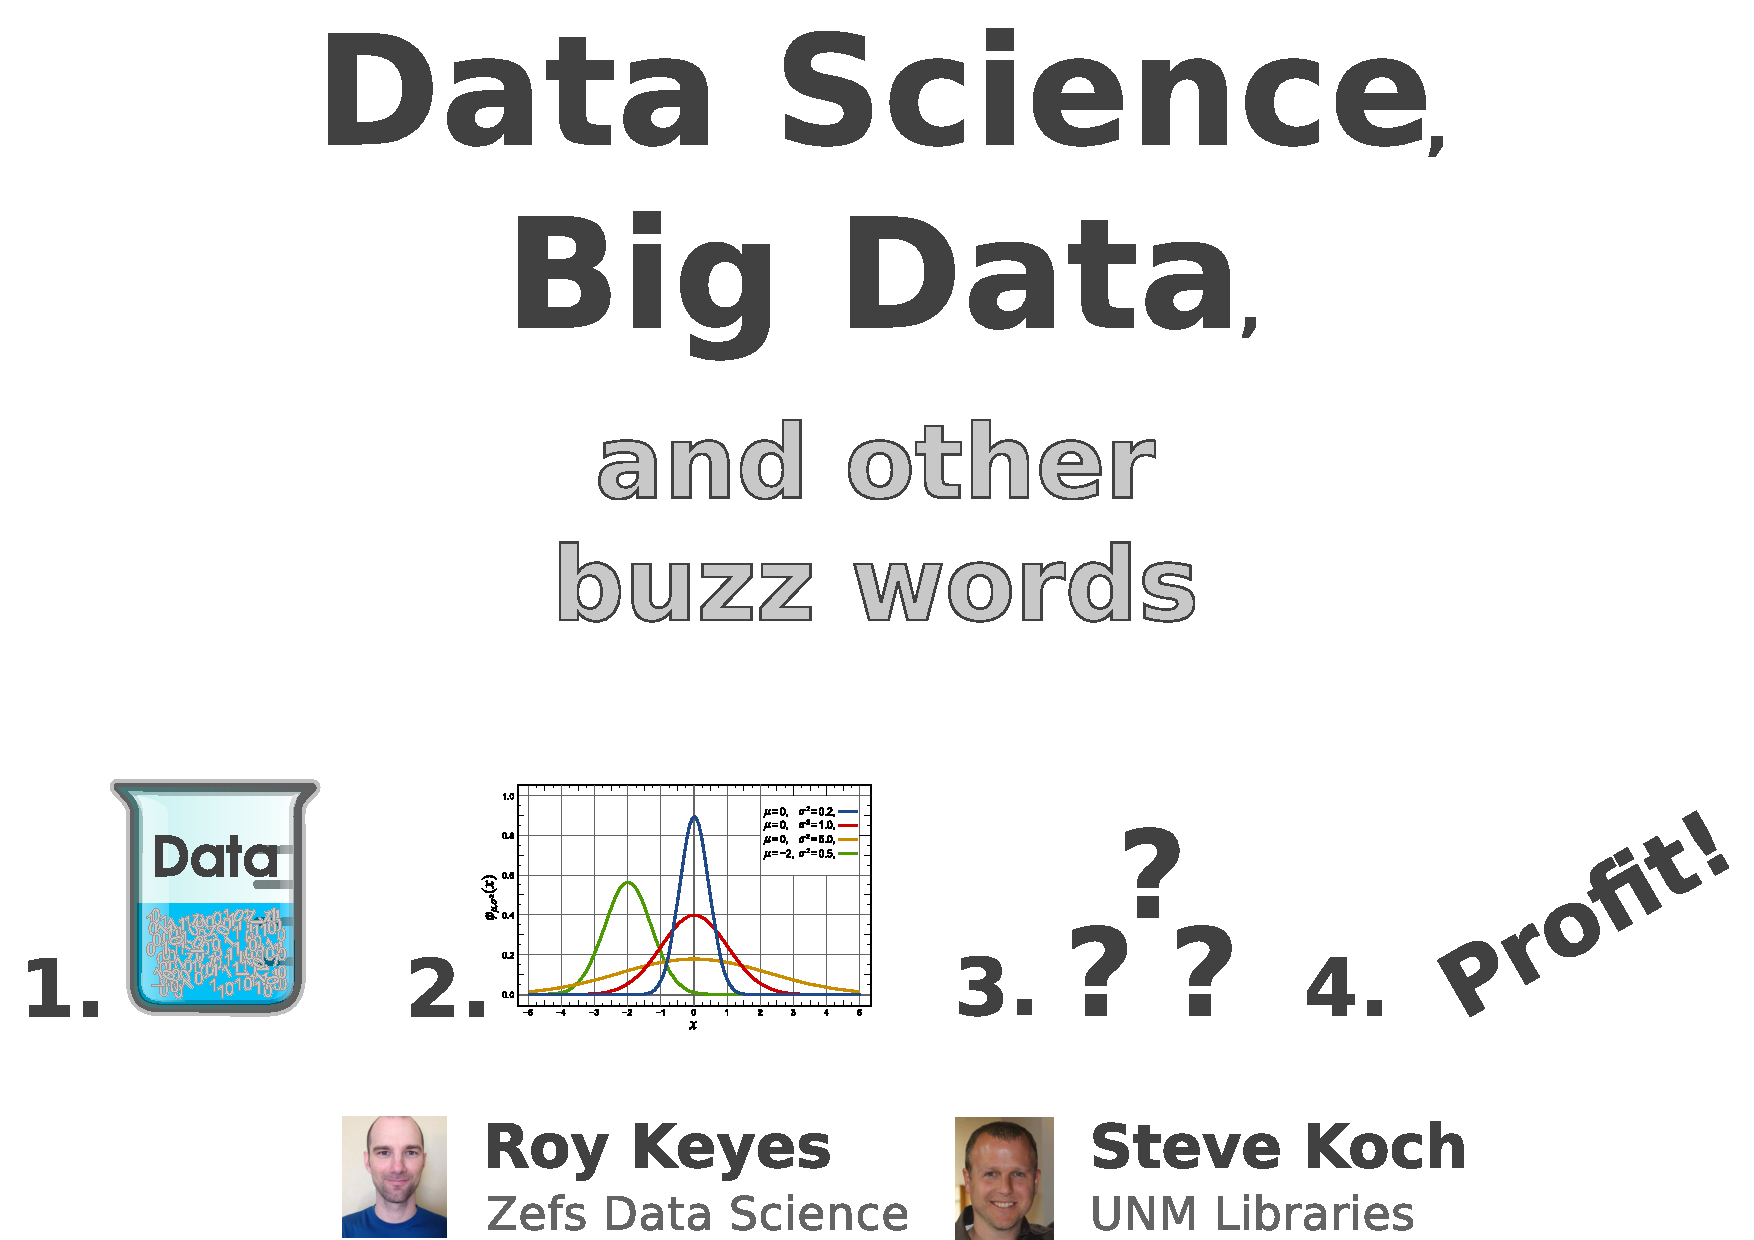
\includegraphics[width=1.0\textwidth]{graphics/data_title2.pdf}
\end{center}
}

%%%%%%%%%%%%%%%%%%%%%%%%%%%%%%%%%%%%%%%%%%%%%%%%%%%%%%%%%%%%%%%%%%%%%%%%%%%%%%%%%%%%%%%%%%%%%%%%%

\begin{frame}
%\frametitle{Suddenly data is everywhere!}
\begin{center}
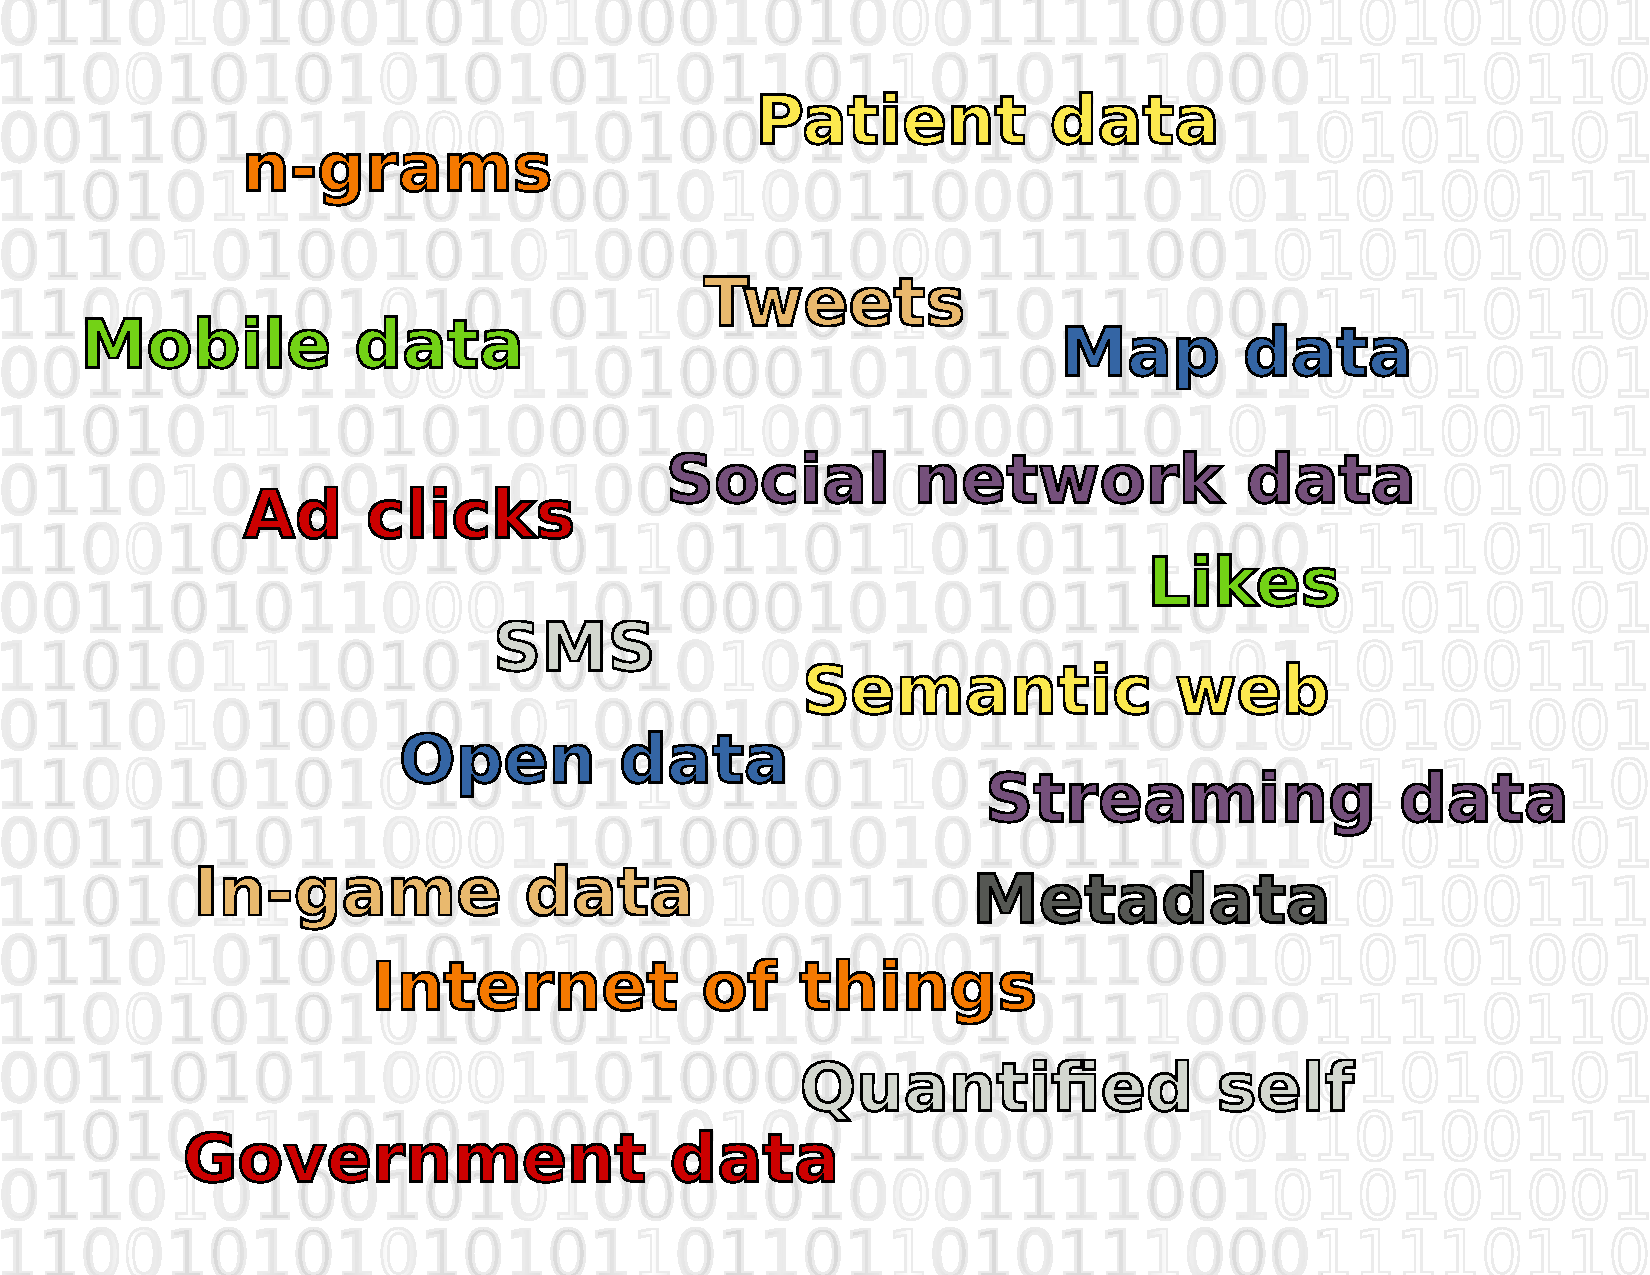
\includegraphics[width=1\textwidth]{graphics/data_cloud2.pdf}
\end{center}
\end{frame}

%%%%%%%%%%%%%%%%%%%%%%%%%%%%%%%%%%%%%%%%%%%%%%%%%%%%%%%%%%%%%%%%%%%%%%%%%%%%%%%%%%%%%%%%%%%%%%%%%

\begin{frame}
\frametitle{Data data data}

\begin{center}

\begin{columns}

\begin{column}{0.5\textwidth}
\begin{center}
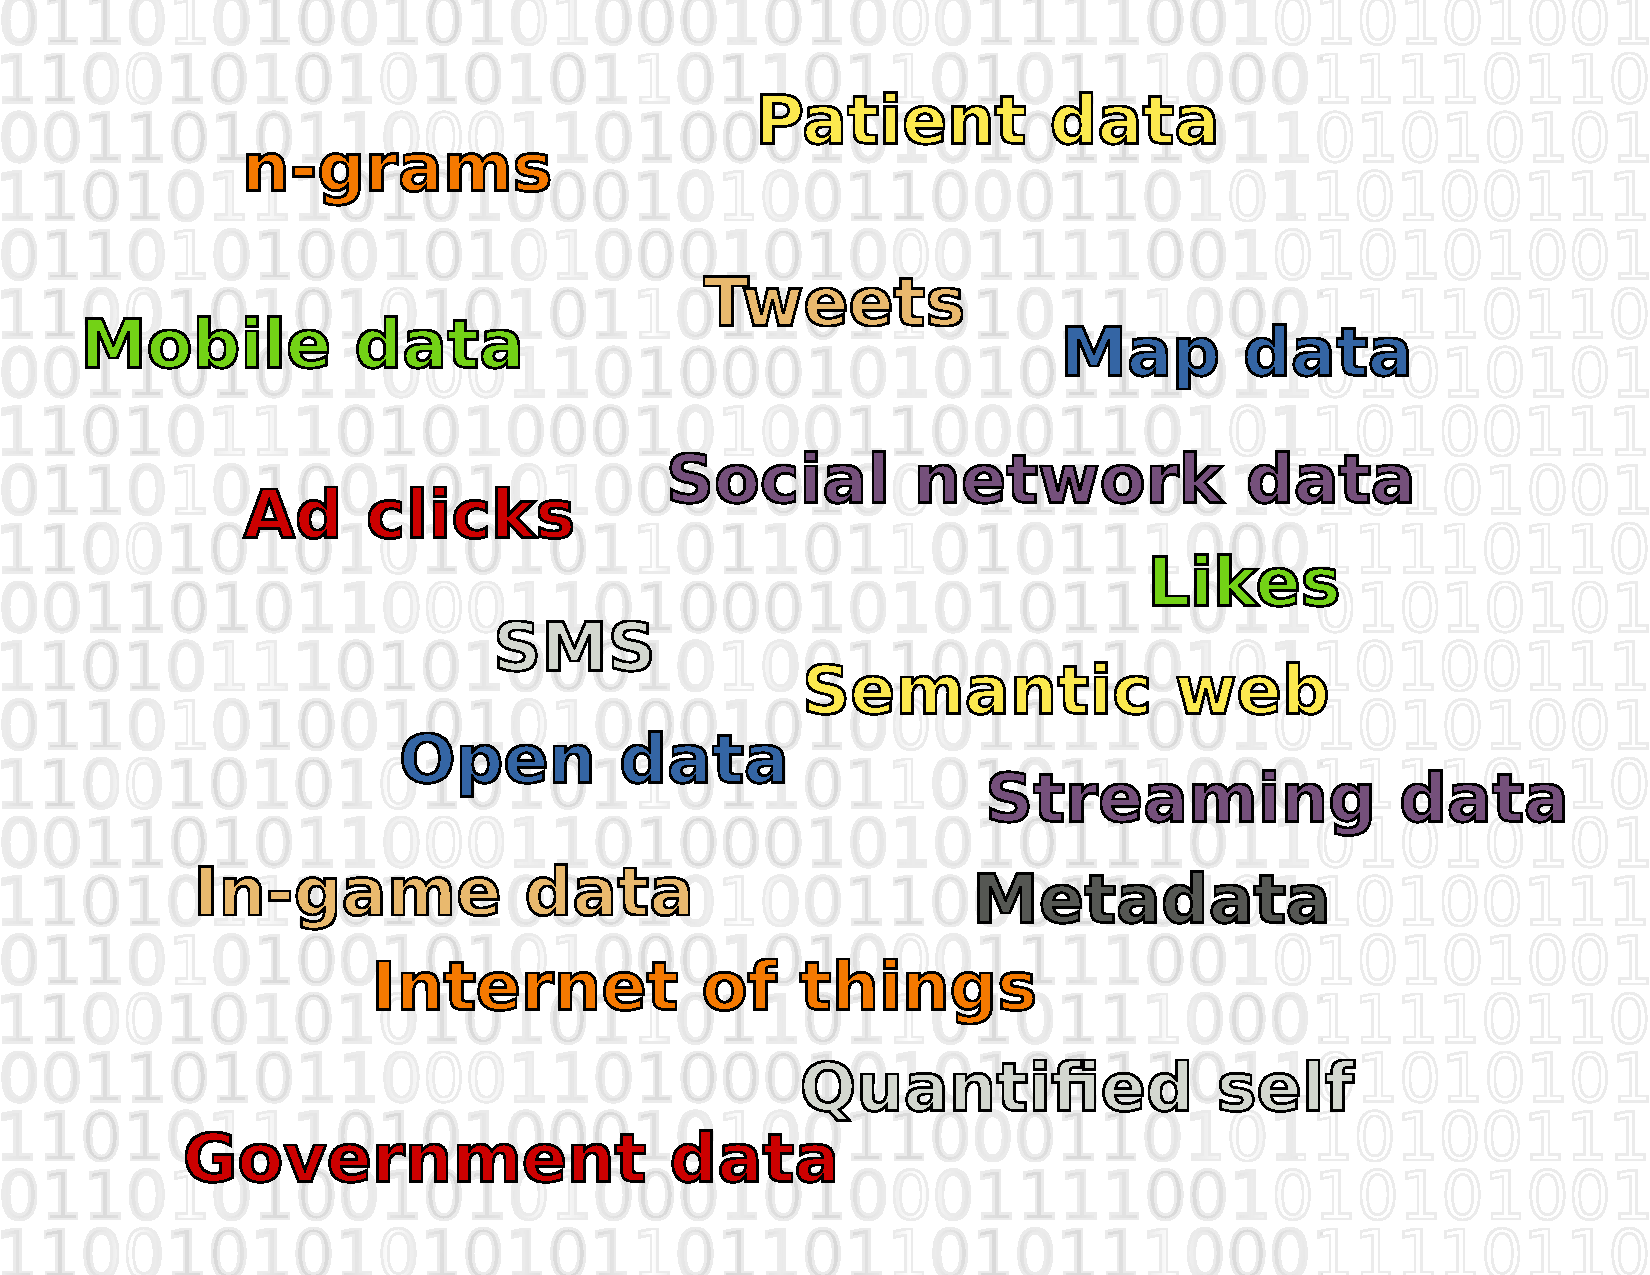
\includegraphics[width=0.7\textwidth]{graphics/data_cloud2.pdf}\\
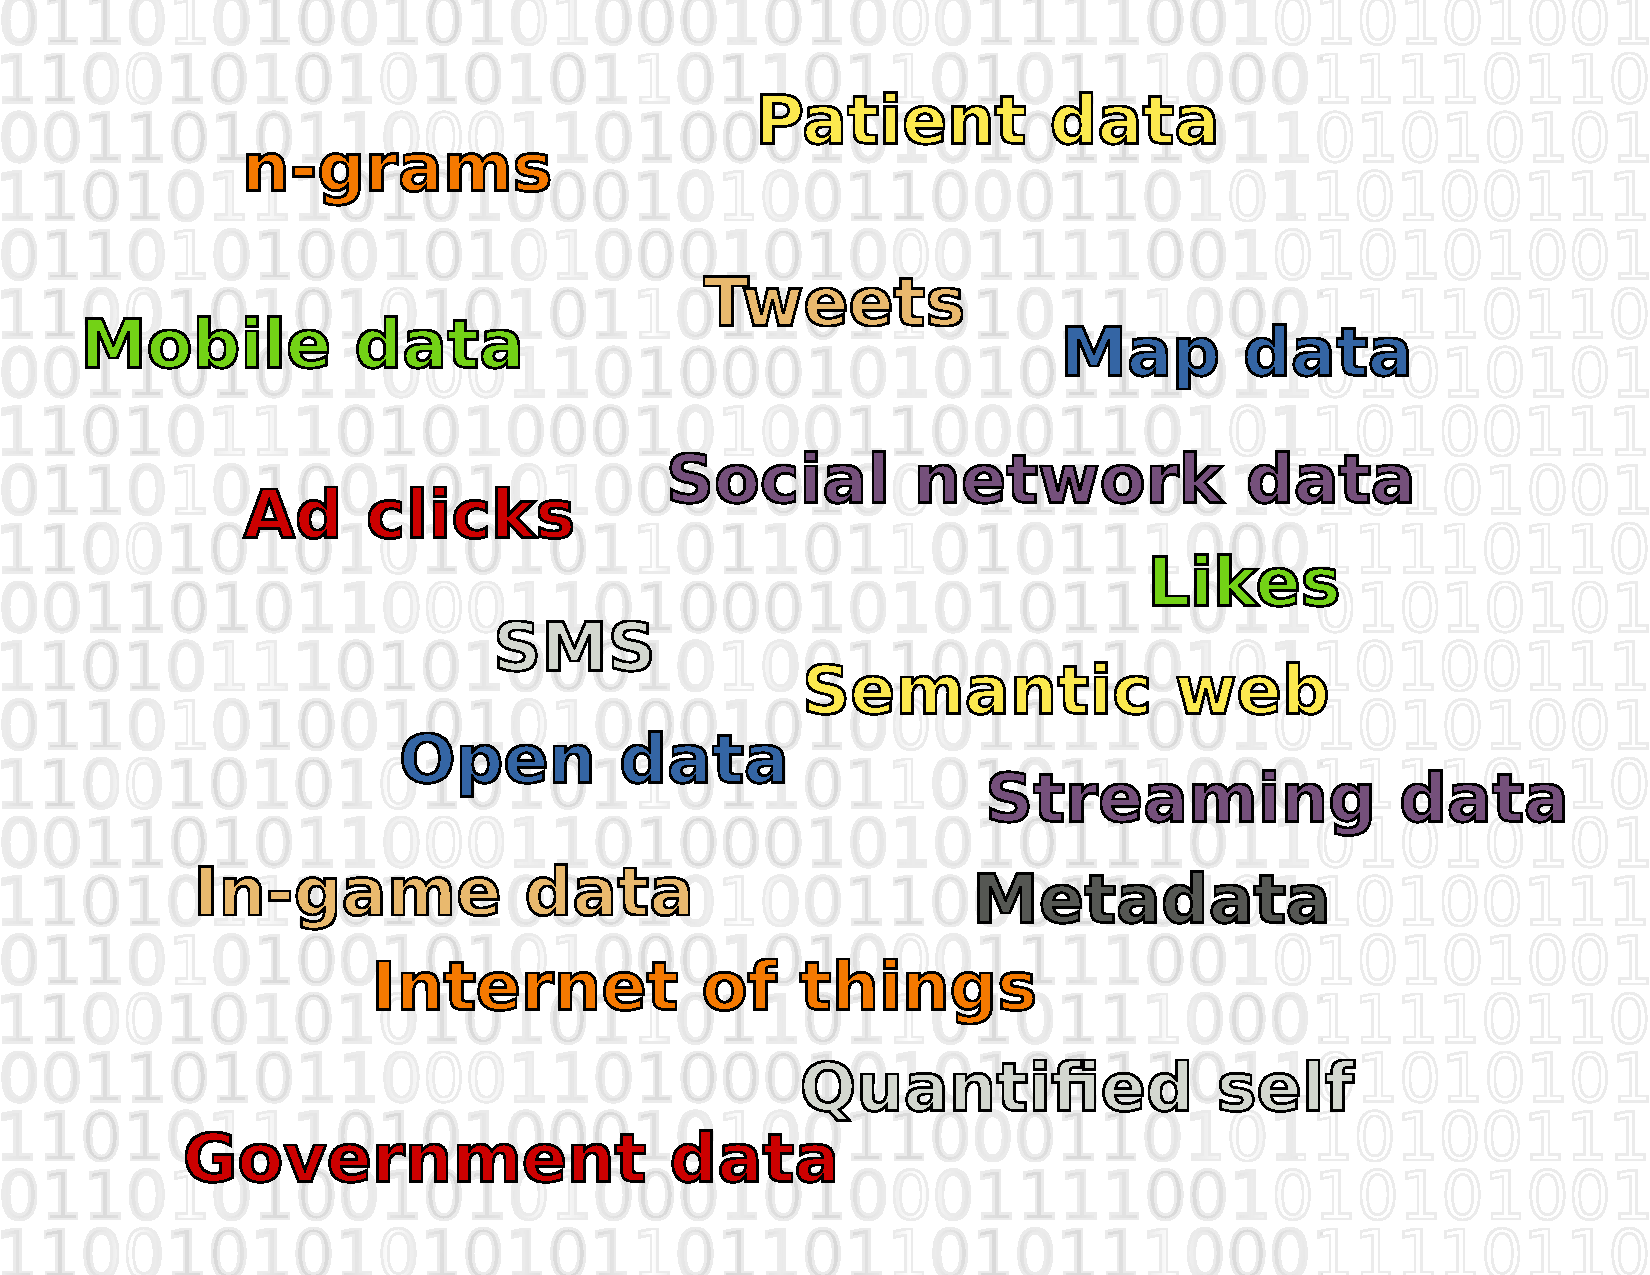
\includegraphics[width=0.7\textwidth]{graphics/data_cloud2.pdf}\\
\bigskip
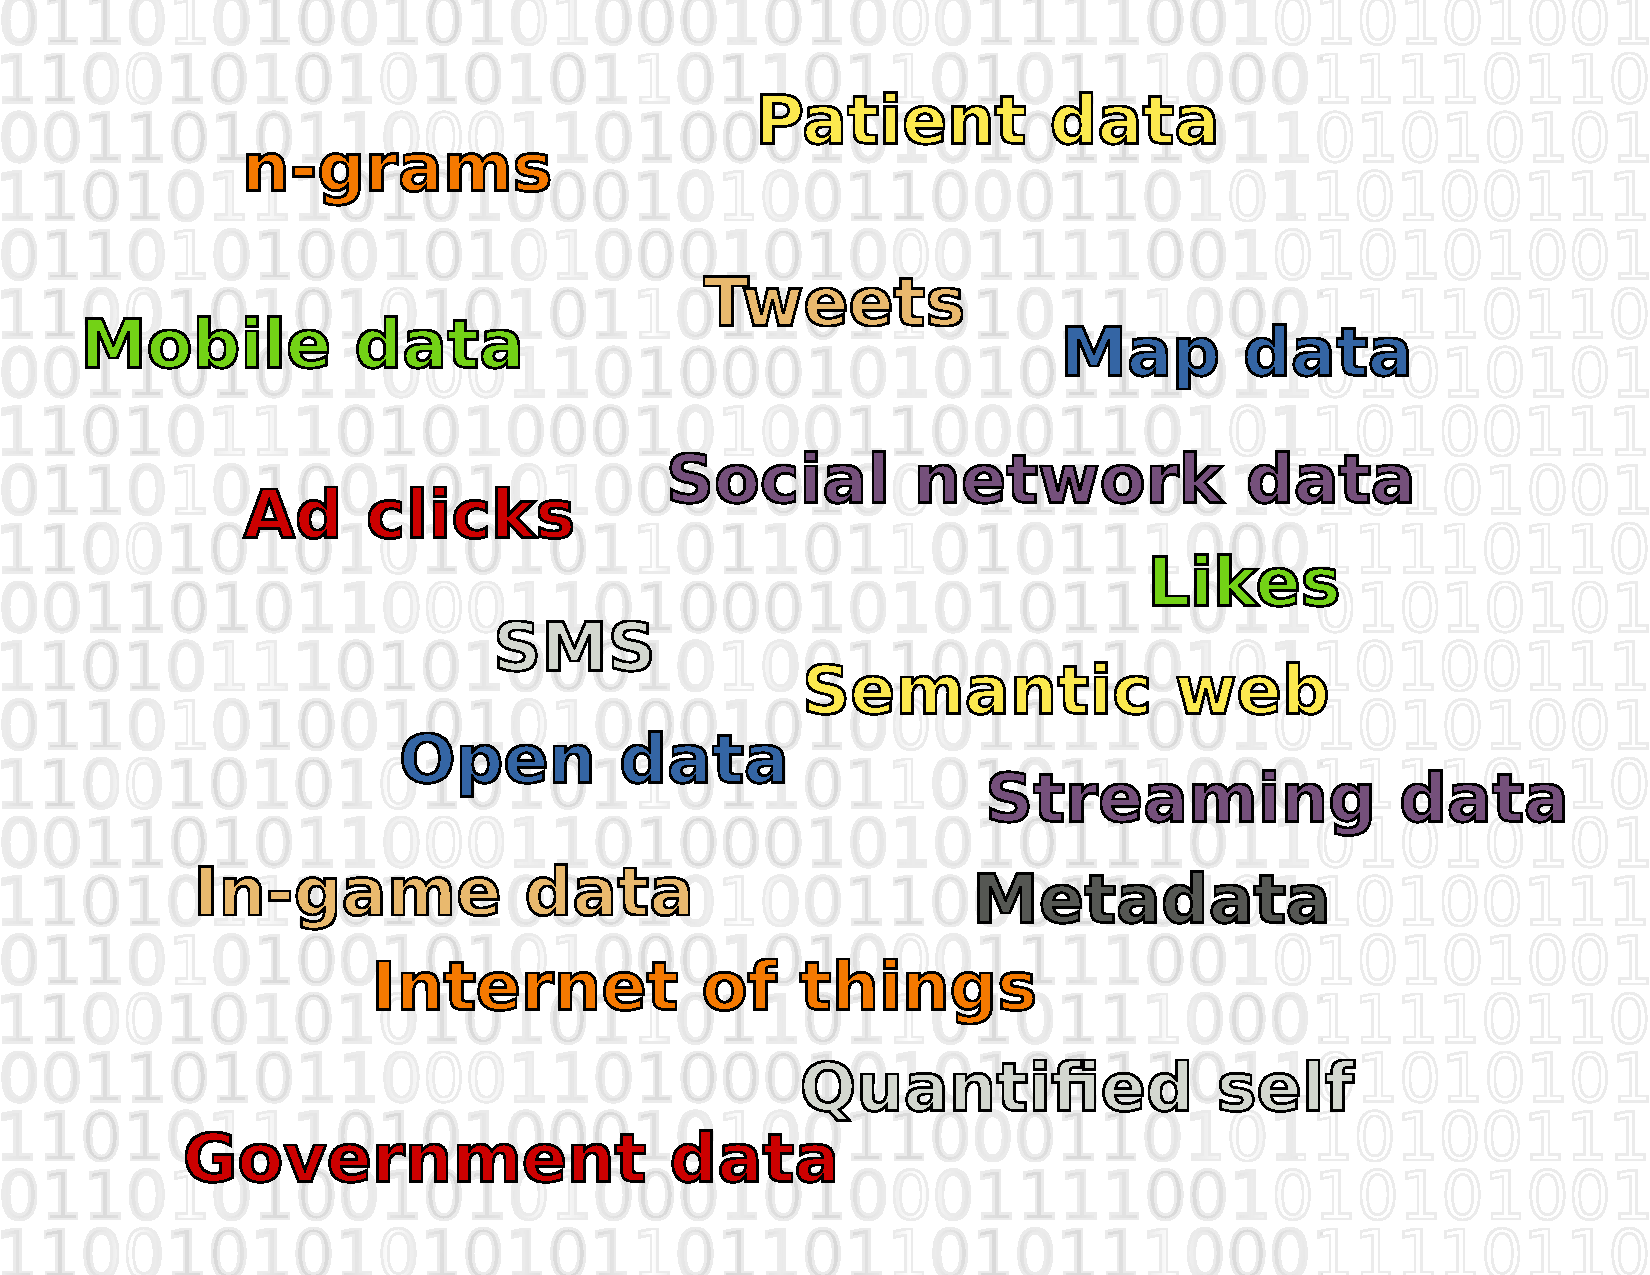
\includegraphics[width=0.7\textwidth]{graphics/data_cloud2.pdf}
\end{center}
\end{column}

\begin{column}{0.5\textwidth}
Data.\\
\bigskip
\bigskip
\bigskip

More data.\\
\bigskip
\bigskip
\bigskip

Even more data.
\end{column}

\end{columns}

\end{center}

\end{frame}

%%%%%%%%%%%%%%%%%%%%%%%%%%%%%%%%%%%%%%%%%%%%%%%%%%%%%%%%%%%%%%%%%%%%%%%%%%%%%%%%%%%%%%%%%%%%%%%%

\begin{frame}
\frametitle{The Data data}

\begin{center}
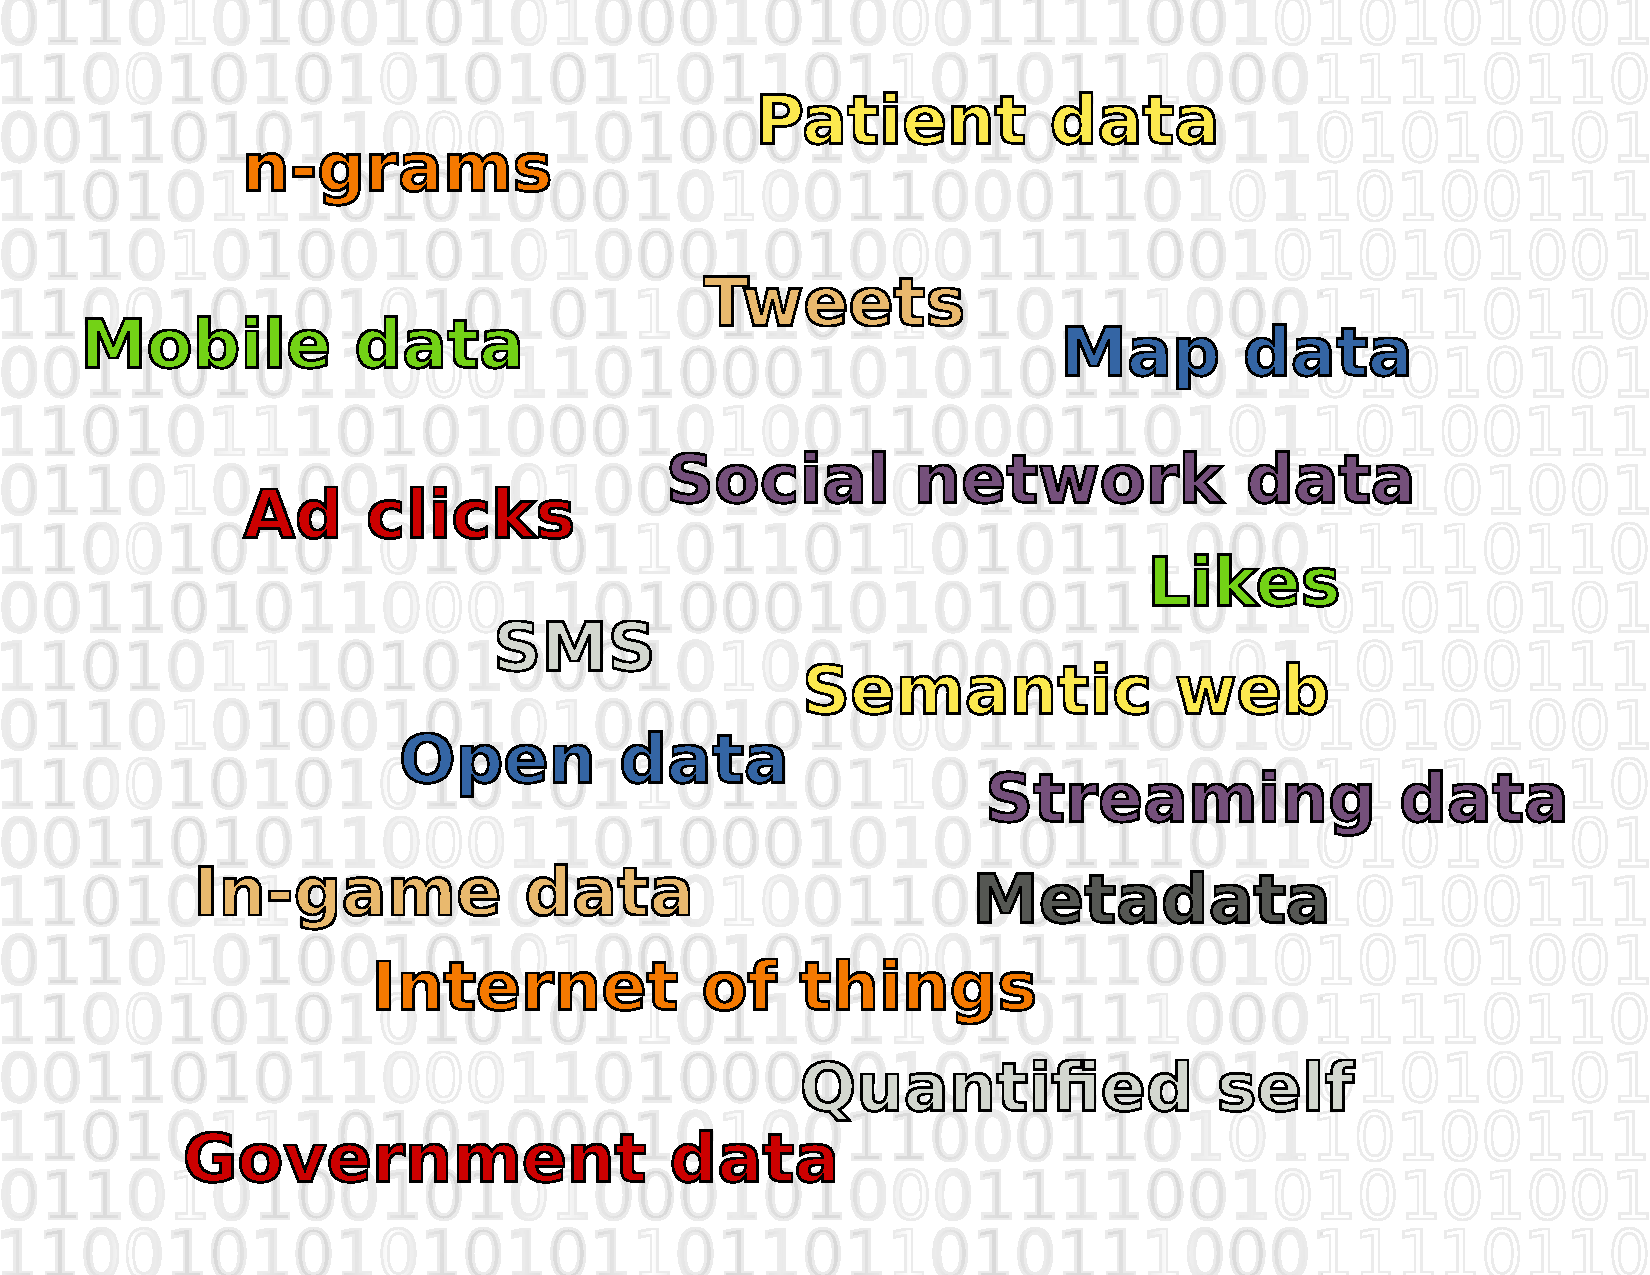
\includegraphics[width=0.3\textwidth]{graphics/data_cloud2.pdf}

\begin{columns}

\begin{column}{0.5\textwidth}
\begin{center}
\begin{itemize}
\item Data, data, data.
\item Data is data.
\end{itemize}
\end{center}
\end{column}

\begin{column}{0.5\textwidth}
\begin{itemize}
\item Data will outperform data.
\item Data determines data.
\item Data + data = data.
\end{itemize}
\end{column}

\end{columns}

\end{center}

\end{frame}

%%%%%%%%%%%%%%%%%%%%%%%%%%%%%%%%%%%%%%%%%%%%%%%%%%%%%%%%%%%%%%%%%%%%%%%%%%%%%%%%%%%%%%%%%%%%%%%%%

\begin{frame}
\frametitle{Data by bullet points}
\begin{center}

\begin{block}{Data by bullet points}
\begin{itemize}
	\item Data is best described by bullet points.
	\item Bullet points are best used in boxes.
	\item Boxes are best.
\end{itemize}
\end{block}

\begin{exampleblock}{More bullet points}
\begin{itemize}
	\item More bullet points are even better.
	\item Better is the next level of goodness.
	\item Data = good.
\end{itemize}
\end{exampleblock}

\end{center}
\end{frame}

%%%%%%%%%%%%%%%%%%%%%%%%%%%%%%%%%%%%%%%%%%%%%%%%%%%%%%%%%%%%%%%%%%%%%%%%%%%%%%%%%%%%%%%%%%%%%%%%%

\end{document}
